\documentclass[10pt]{beamer}
\usetheme[
%%% option passed to the outer theme
%    progressstyle=fixedCircCnt,   % fixedCircCnt, movingCircCnt (moving is deault)
  ]{Feather}
  
% If you want to change the colors of the various elements in the theme, edit and uncomment the following lines

% Change the bar colors:
%\setbeamercolor{Feather}{fg=red!20,bg=red}

% Change the color of the structural elements:
%\setbeamercolor{structure}{fg=red}

% Change the frame title text color:
%\setbeamercolor{frametitle}{fg=blue}

% Change the normal text color background:
%\setbeamercolor{normal text}{fg=black,bg=gray!10}

%-------------------------------------------------------
% INCLUDE PACKAGES
%-------------------------------------------------------

\usepackage[utf8]{inputenc}
\usepackage[english]{babel}
\usepackage[T1]{fontenc}
\usepackage{helvet}

%-------------------------------------------------------
% DEFFINING AND REDEFINING COMMANDS
%-------------------------------------------------------

% colored hyperlinks
\newcommand{\chref}[2]{
  \href{#1}{{\usebeamercolor[bg]{Feather}#2}}
}

%-------------------------------------------------------
% INFORMATION IN THE TITLE PAGE
%-------------------------------------------------------

\title[] % [] is optional - is placed on the bottom of the sidebar on every slide
{ % is placed on the title page
      \textbf{Operating Systems, What's broken?}
}

\subtitle[Operating Systems, What's broken?]
{
}

\author[Rodrigo Siqueira Jordão]
{      Rodrigo Siqueira Jordão \\
      {\ttfamily siqueira@kuniri.org}
}

\institute[]
{
      Institute of Mathematics and Statistics\\
      University of Sao Paulo\\
  
  %there must be an empty line above this line - otherwise some unwanted space
  % is added between the university and the country (I do not know why;( )
}

\date{\today}

%-------------------------------------------------------
% THE BODY OF THE PRESENTATION
%-------------------------------------------------------

\begin{document}

%-------------------------------------------------------
% THE TITLEPAGE
%-------------------------------------------------------

{\1% % this is the name of the PDF file for the background
% the plain option removes the header from the title page, noframenumbering removes the numbering of this frame only
\begin{frame}[plain,noframenumbering] 
  \titlepage % call the title page information from above
\end{frame}}

\begin{frame}{Content}{}
  \tableofcontents
\end{frame}

%=======================================================
\section{Introduction}
%=======================================================
\begin{frame}{Introduction}
%-------------------------------------------------------
  \begin{figure}[ht]
    \vspace{5pt}
    \centering
    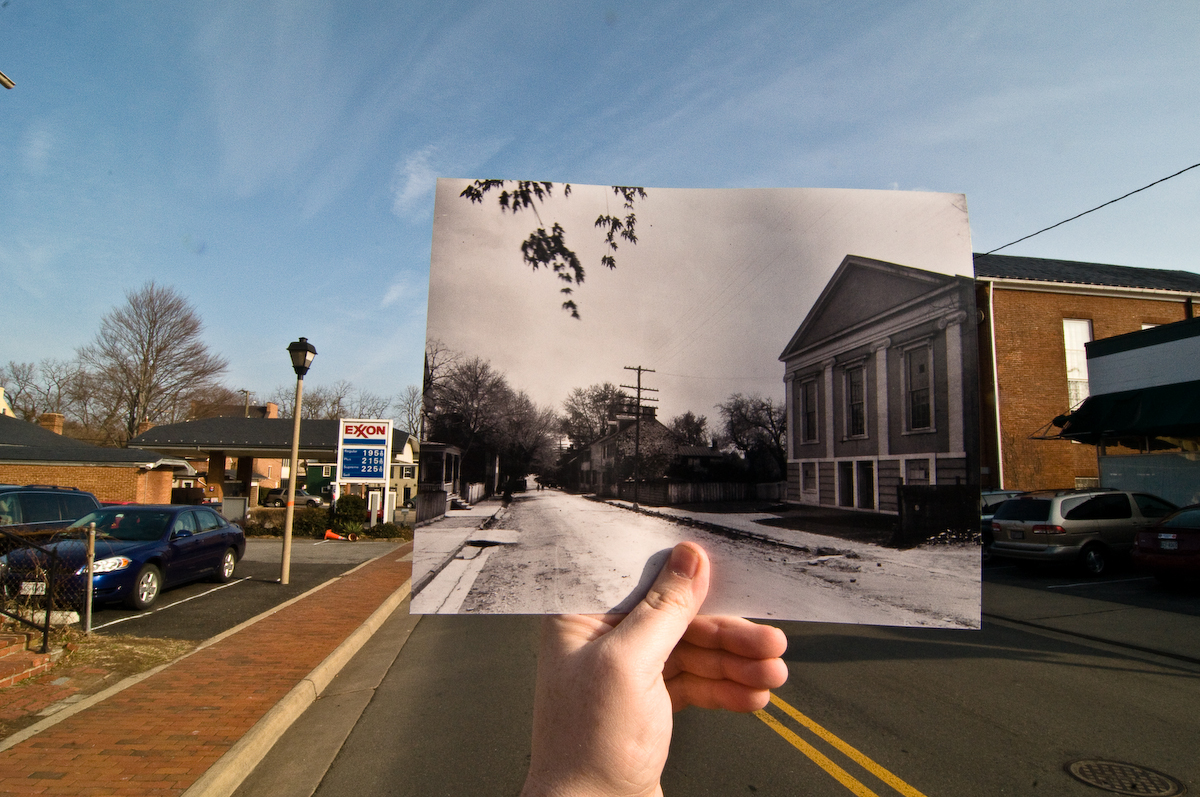
\includegraphics[width=1\textwidth, keepaspectratio=true]{images/designwontchange.jpg}
    \caption {Design won't change}
    \label {assembler}
  \end{figure}
\end{frame}

%-------------------------------------------------------
\begin{frame}{OS design won't change}
%-------------------------------------------------------
  \begin{itemize}
    \item Requirement for backward compatibility; \pause
    \item UNIX model's historical resilience and; \pause
    \item If it ain't broke, don't fix it.
  \end{itemize}
\end{frame}

%-------------------------------------------------------
\begin{frame}{Innovators Dilemma}{Introduction}
%-------------------------------------------------------

  \begin{block}{Innovators Dilemma}
  A variety of interests have invested substantially in current OS structures
  and view disruption with suspicion.
  \end{block}

  \begin{figure}[ht]
    \hspace{-120pt}
    
\includegraphics[width=0.5\textwidth, keepaspectratio=true]{images/frysuspicious.jpg}
  \end{figure}

\end{frame}

\begin{frame}{Technical}{Introduction}
%-------------------------------------------------------
  \begin{block}{Technical}
  By following the argument that OS will change, we can identify the
  most promising paths for OS research.
  \end{block}

  \begin{figure}[ht]
    \hspace{100pt}
    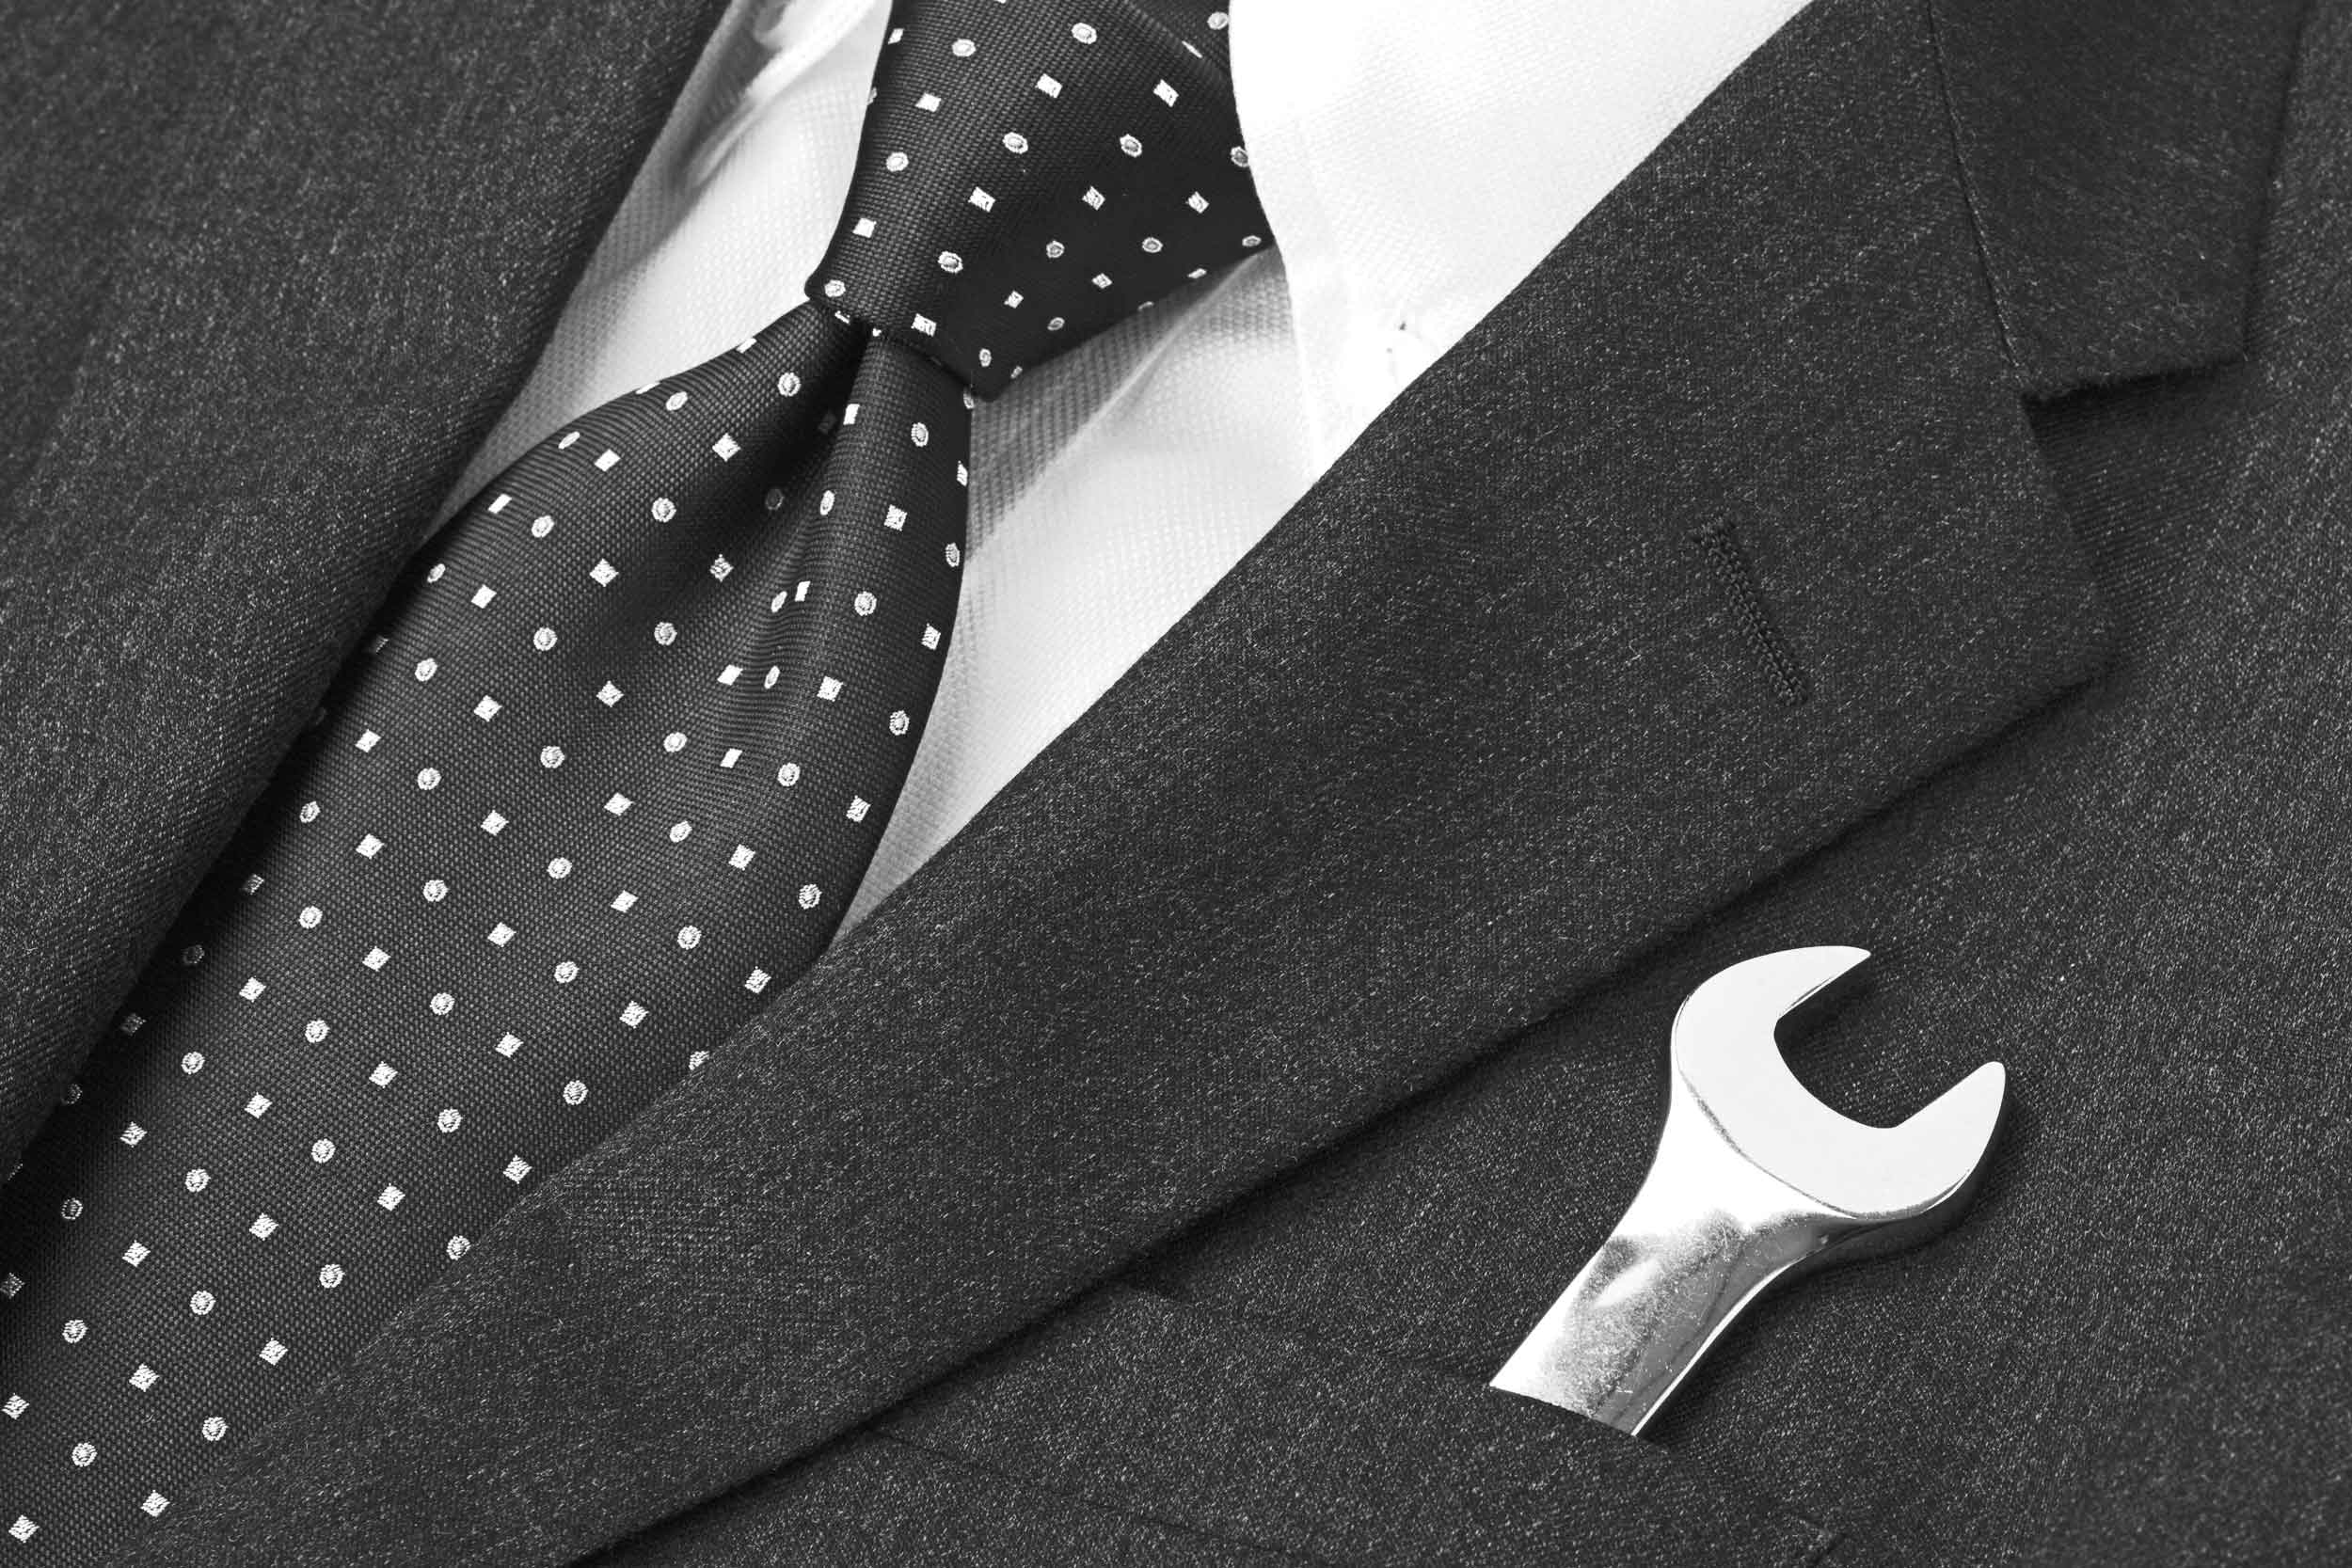
\includegraphics[width=0.5\textwidth, keepaspectratio=true]{images/technical.jpg}
  \end{figure}

\end{frame}

%=======================================================
\section{Hardware trends}
\begin{frame}{Hardware trends}

  \begin{figure}[ht]
    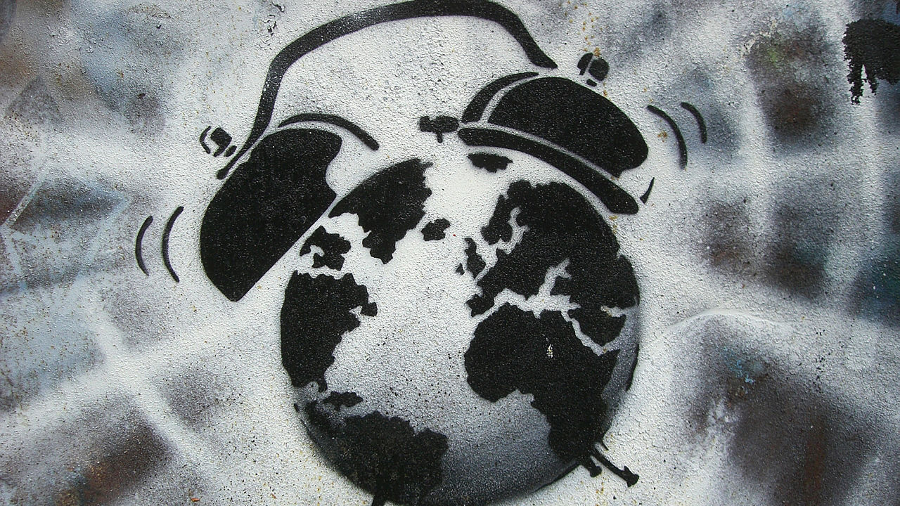
\includegraphics[width=0.7\textwidth, keepaspectratio=true]{images/hwAndAppChangeFast.png}
  \end{figure}\pause

  \begin{block}{}
  Hardware is changing at the levels of individual devices, cores, board and
  complete computer systems.
  \end{block}

\end{frame}
%-------------------------------------------------------
\subsection{Complexity}

\begin{frame}{Complexity}{Hardware trends}

  \begin{figure}[ht]
    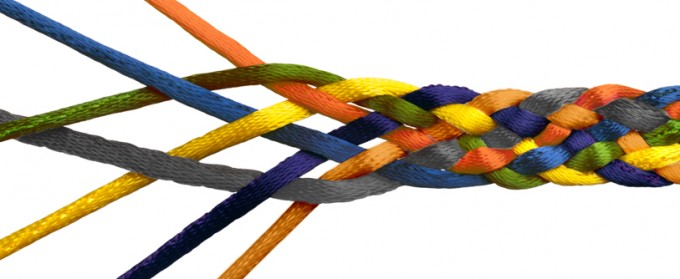
\includegraphics[width=0.5\textwidth, keepaspectratio=true]{images/integrated.jpg}
  \end{figure}\pause

  \begin{itemize}
    \item Large number of peripheral devices are integrated onto a die, each
          with complex, varying programming models; \pause
    \item More and more of these devices are now built as specialized processor
          that execute specialized firmware with little OS integration; \pause
    \item The view of computer as a single cache-coherent physical address
          space containing RAM and devices has been a myth for at least the
          last decade.
  \end{itemize}
\end{frame}

%-------------------------------------------------------
\subsection{Energy}
\begin{frame}{Energy}{Hardware trends}
%-------------------------------------------------------
  \begin{figure}[ht]
    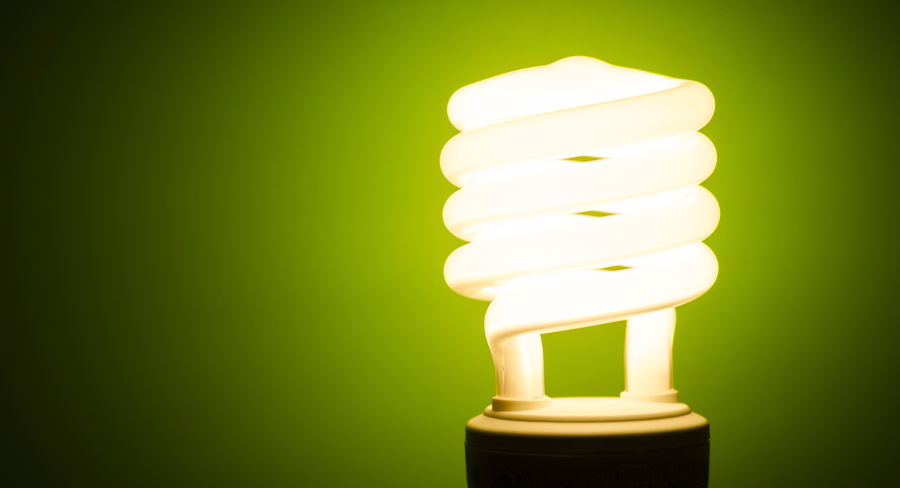
\includegraphics[width=0.5\textwidth, keepaspectratio=true]{images/energy.png}
  \end{figure} \pause

  \begin{itemize}
    \item As a system resource to be managed by the OS, energy is now just as
          important as CPU cycles. \pause
    \item New OS design is that most of the hardware, can be powered up and
          down at any point during execution.
  \end{itemize}
\end{frame}


%-------------------------------------------------------
\subsection{Nonvolatile main memory}
\begin{frame}{Nonvolatile main memory}{Hardware trends}
%-------------------------------------------------------
  \begin{columns}[T] % align columns
    \begin{column}{.2\textwidth}
      \begin{figure}[ht]
        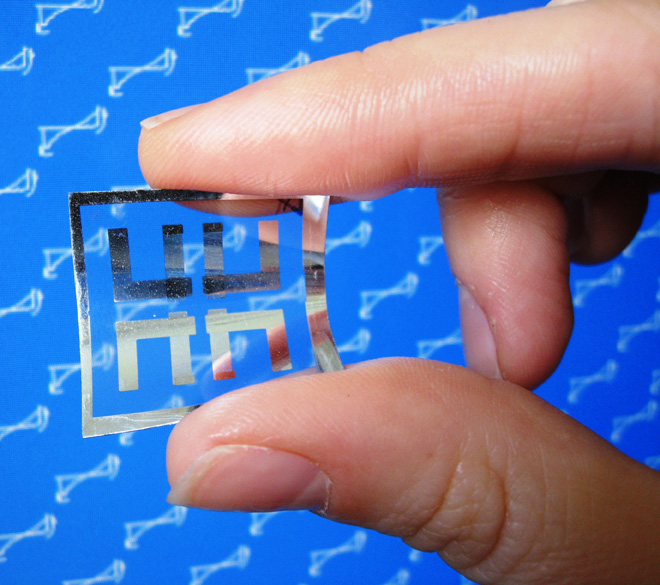
\includegraphics[width=1.8\textwidth, keepaspectratio=true]{images/nvm.jpg}
      \end{figure} \pause
    \end{column}%

    \hfill%
    \begin{column}{.7\textwidth}
      \begin{itemize}
        \item Nonvolatile main memories to become prevalent.
        \begin{itemize}
          \item Packaging, cost, and power efficiency will make it possible to
                architect and deploy far more nonvolatile RAM.\pause
        \end{itemize}
        \item With large numbers of heterogeneous processors, this memory will be
              highly distributed but perhaps not in the way we see today.\pause
          \begin{itemize}
            \item Photonic interconnects
            \item High-radix
          \end{itemize}\pause
        \item In the longer term, memory controllers are likely to become more
              intelligent and programmable at the OS level.
      \end{itemize}
    \end{column}%
\end{columns}
\end{frame}

%-------------------------------------------------------
\subsection{System}
\begin{frame}{System}{Hardware trends}
%-------------------------------------------------------
  \begin{figure}[ht]
    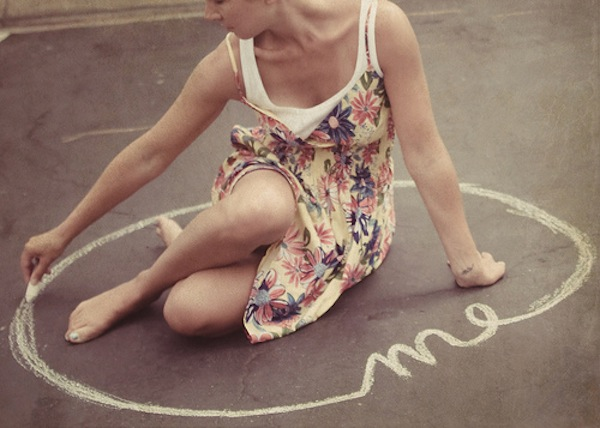
\includegraphics[width=0.6\textwidth, keepaspectratio=true]{images/boundary.jpg}
  \end{figure} \pause

  \begin{block}{}
    Boundaries of today's machine are different from traditional scale-up and
    scale-out systems.
   \end{block}
\end{frame}

%-------------------------------------------------------
\subsection{Diversity}
\begin{frame}{Diversity}{Hardware trends}
%-------------------------------------------------------
  \begin{figure}[ht]
    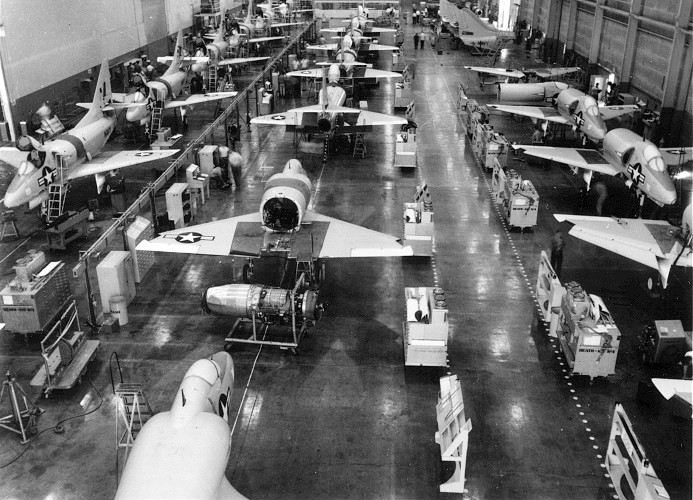
\includegraphics[width=0.4\textwidth, keepaspectratio=true]{images/diversity.jpg}
  \end{figure} \pause

  \begin{itemize}
    \item SoC were always heterogeneous, but they were used in special-purpose
          systems; now they were used in general-purpose systems.\pause
      \begin{itemize}
        \item ``Engineering a general-purpose OS that can be used widely and
             evolve as hardware as hardware changes is a formidable challenge''
      \end{itemize}\pause
    \item Hardware adapts and diversifies much faster today than system does.
   \end{itemize}
\end{frame}

%=======================================================
\section{Application Changes}
\begin{frame}{Application Changes}
%-------------------------------------------------------
  \begin{figure}[ht]
    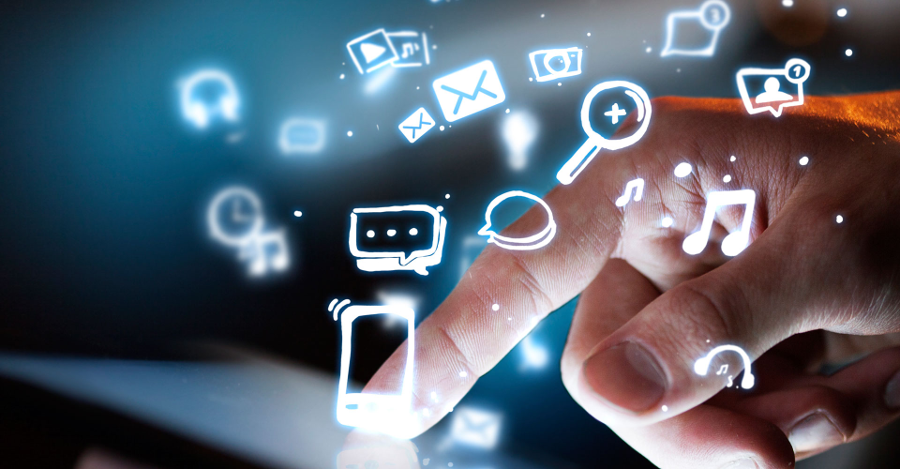
\includegraphics[width=0.9\textwidth, keepaspectratio=true]{images/application.png}
  \end{figure}

  \begin{block}{}
    The ways in which computers are used and the application that run on them
    are also changing:
  \end{block}
\end{frame}

\begin{frame}{Application Changes}{Challenge}
%-------------------------------------------------------
  \begin{columns}[T] % align columns
    \begin{column}{.2\textwidth}
      \begin{figure}[ht]
        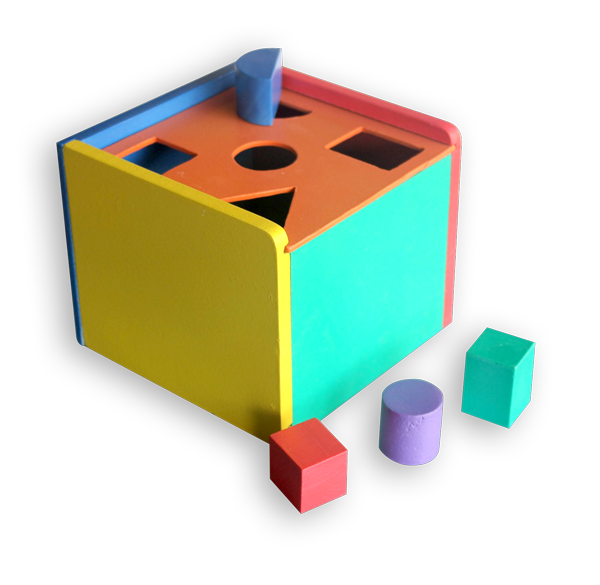
\includegraphics[width=1.5\textwidth, keepaspectratio=true]{images/challenge.png}
      \end{figure}
    \end{column}

    \hfill
    \begin{column}{.7\textwidth}
      \begin{block}{Challenge}
        Current OSs don't match up well with the applications they're called on to
        support.
      \end{block}
    \end{column}
  \end{columns}
\end{frame}

\begin{frame}{Application Changes}{Opportunity}
%-------------------------------------------------------
  \begin{columns}[T] % align columns
    \begin{column}{.5\textwidth}
      \begin{block}{Opportunity}
        The burden of history is light. Applications are very different now,
        granting us the freedom to change the OS interface.
      \end{block}
    \end{column}

    \hfill
    \begin{column}{.4\textwidth}
      \begin{figure}[ht]
        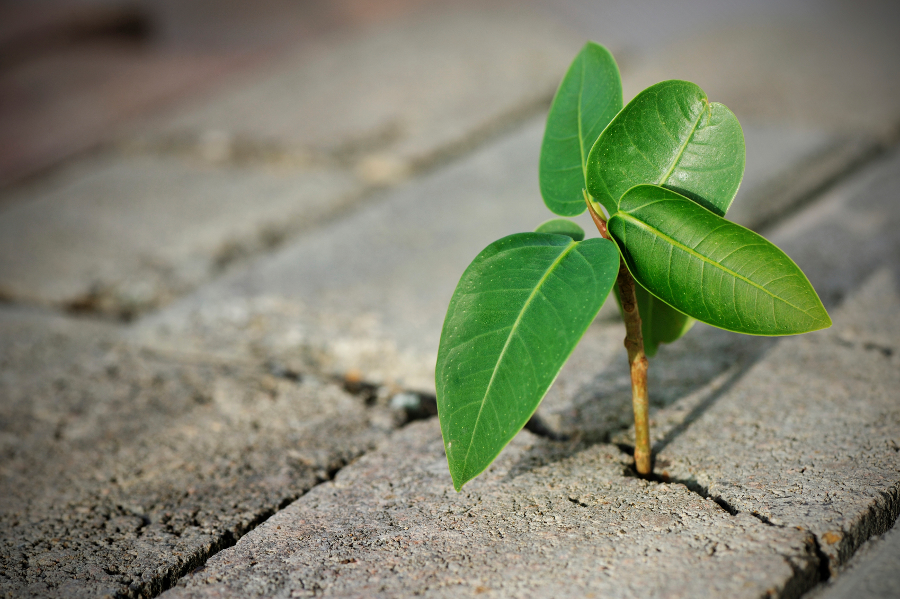
\includegraphics[width=1\textwidth, keepaspectratio=true]{images/opportunity.png}
      \end{figure}
    \end{column}
  \end{columns}

\end{frame}

%-------------------------------------------------------
\subsection{Rack-scale}
\begin{frame}{Rack-scale}{Application Changes}
%-------------------------------------------------------
  \begin{itemize}
    \item It's the next step of cloud computing.
    \begin{itemize}
      \item The authors seeing a new trend: deploy software as appliances
            (tin-wrapped) in a rack-scale.
      \item "Rack-scale: it is a big step by re-architecting cloud platform"
    \end{itemize}
    \item Appliances usually consist of a collection of server machines and
          optional custom hardware accelerators, connected by a high-bandwidth
          internal network such as infiniband.
    \item Tin-wrapped software, is attractive to software vendor by two main
          reasons:
      \begin{enumerate}
        \item Vendor controls the hardware platform that the OS runs on,
               support cost are greatly reduced.
        \item Software also allows vendors to introduce custom hardware that
              doesn't have to be compatible with every customer's existing
              systems.
      \end{enumerate}
    \item Rack-scale application often exploit the lowest-latency communication
          mechanisms available, such as RDMA.
  \end{itemize}
\end{frame}

%-------------------------------------------------------
\subsection{Datacenter challenges}
\begin{frame}{Datacenter challenges}{Application Changes}
%-------------------------------------------------------
  \begin{figure}[ht]
    \centering
    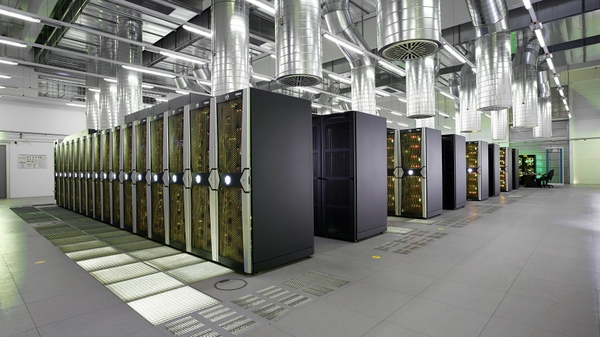
\includegraphics[width=1\textwidth, keepaspectratio=true]{images/datacenter.jpg}
  \end{figure}
\end{frame}

\begin{frame}{Datacenter challenges}{Application Changes}
%-------------------------------------------------------
  \begin{enumerate}
    \item Application deployment, upgrades, and maintenance. \pause
    \item Code must be upgraded across thousands of machines in a coordinated
          manner, often without suffering from down. \pause
    \item Cloud service in datacenter often have much more complex requirement
          from the infrastructure. \pause
     \begin{itemize}
      \item Increase in software - Defined network (SDN). \pause
     \end{itemize}
    \item Application security requirements have also radically changed. \pause
    \item Application increasingly span centralized data center services.
  \end{enumerate}
\end{frame}

%=======================================================
\section{What's broken?}
%-------------------------------------------------------
\begin{frame}{What's broken?}{}
%-------------------------------------------------------
  \begin{figure}[ht]
    \centering
    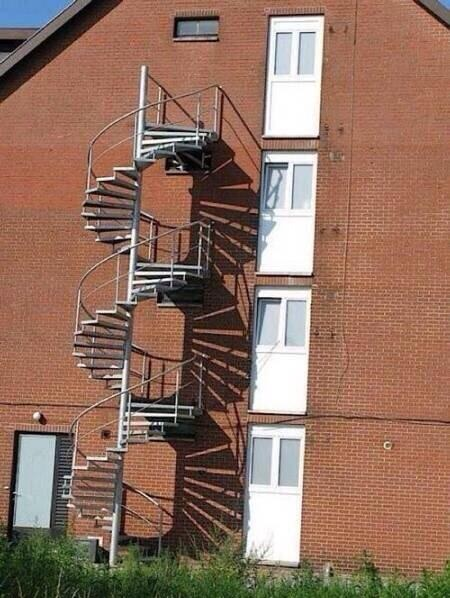
\includegraphics[width=0.5\textwidth, keepaspectratio=true]{images/whatsbroken.jpg}
  \end{figure}
\end{frame}
%------------------------------------------------------
\begin{frame}{What's broken?}
%-------------------------------------------------------
  \begin{block}{}
    The real problem is: The fundamental concept are outdated.
  \end{block} \pause

  \begin{block}{}
    It's remarkable how many assumptions about OS design embodied in
    modern system like GNU/Linux and Windows are either violated or
    irrelevant.
  \end{block}

  \begin{block}{}
    What will such an OS look like?
  \end{block}
\end{frame}

%-------------------------------------------------------
\subsection{Single monolithic kernel}
%-------------------------------------------------------
\begin{frame}{Single monolithic kernel}{What's broken?}
%-------------------------------------------------------
  \begin{columns}[T]
    \begin{column}{.3\textwidth}
      \begin{figure}[ht]
        \centering
        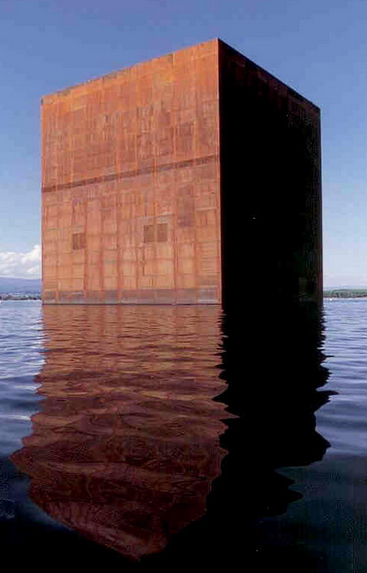
\includegraphics[width=0.7\textwidth, keepaspectratio=true]{images/monolith.png}
      \end{figure}
    \end{column} \pause

    \hfill
    \begin{column}{.7\textwidth}
      \begin{block}{}
        Concepts at modern OS.
      \end{block} \pause

      \begin{itemize}
        \item Single, multithreaded; \pause
        \item Shared-memory; \pause
        \item Handle interrupts and system calls.
      \end{itemize}
    \end{column}
  \end{columns}
\end{frame}

\begin{frame}{Single monolithic kernel}{What's broken?}
%-------------------------------------------------------
  \begin{block}{}
    The problem with these concepts:
  \end{block} \pause

  \begin{itemize}
    \item Doesn't work on a machine with heterogeneous processors; \pause
    \item Different instruction sets; \pause
    \item Memory that's not completely coherent; \pause
    \item Exists at different address as seen by different cores; \pause
    \item Current kernels can be trusted with few gigabytes of memory, however
          machines with petabytes of memory can generate failures.
  \end{itemize}

  \begin{block}
    Modern computers Vs. Distributed Systems
  \end{block}
\end{frame}

%-------------------------------------------------------
\subsection{Authorization and security}
%-------------------------------------------------------
\begin{frame}{Authorization and security}{What's broken?}
%-------------------------------------------------------
  \begin{columns}[T]
    \begin{column}{.3\textwidth}
      \begin{figure}[ht]
        \centering
        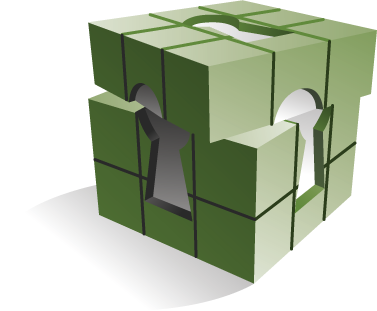
\includegraphics[width=0.8\textwidth, keepaspectratio=true]{images/authorization.png}
      \end{figure}
    \end{column}

    \hfill
    \begin{column}{.7\textwidth}
      \begin{block}{}
        The security challenges we face today:
      \end{block} \pause

      \begin{enumerate}
        \item Privacy; \pause
        \item Information flow; \pause
        \item Untrusted applications running with user privileges; \pause
        \item Social network with billions of users;
      \end{enumerate}
     \end{column}
  \end{columns}

  \begin{block}{}
    A fine-grained authorization mechanism like that afforded by capabilities,
    perhaps combined with a concept of distributed information flow control
    at scale, could be the way forward.
  \end{block}
\end{frame}

%-------------------------------------------------------
\subsection{Scheduling}
%-------------------------------------------------------
\begin{frame}{Scheduling}{What's broken?}
%-------------------------------------------------------
  \begin{columns}[T]
    \begin{column}{.2\textwidth}
      \begin{figure}[ht]
        \centering
        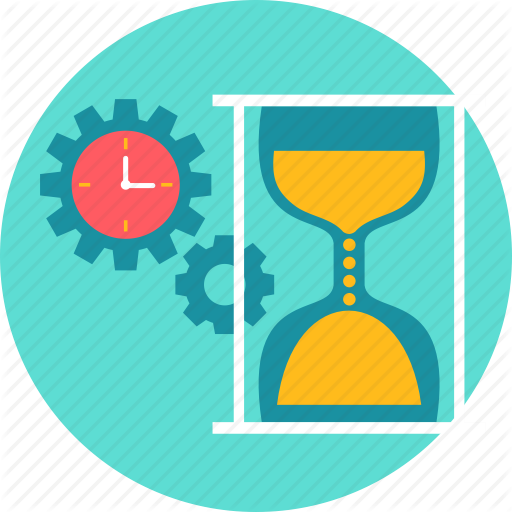
\includegraphics[width=0.6\textwidth, keepaspectratio=true]{images/scheduler.png}
      \end{figure}
    \end{column}

    \hfill
    \begin{column}{.8\textwidth}
      \begin{block}{}
        Modern OS schedulers manage process or threads as basic unit of CPU
        allocation. 
      \end{block} \pause

      \begin{block}{}
        For modern multicore hardware and typical applications this is irrelevant.
      \end{block}
      \end{column}
    \end{columns}
\end{frame}

\begin{frame}{Scheduling}{What's broken?}
  \begin{itemize}
    \item On a single machine, an application spans multiple process and
      threads, and calls out to server process it shares with other
      programs. \pause
    \begin{itemize}
      \item Dynamic migration of threads to balance the load across
            cores makes no sense when cores are radically heterogeneous,
            and where the objective is to optimize energy usage subject
            to fix performance goals.
      \end{itemize} \pause
    \item Effective spatial scheduling, rather than temporal scheduling,
          becomes the key challenge. \pause
      \begin{itemize}
        \item In rack-scale machines, an application is inherently distributed.
      \end{itemize}
    \end{itemize}
\end{frame}

%-------------------------------------------------------
\subsection{Virtual memory}
%-------------------------------------------------------
\begin{frame}{Virtual memory}{What's broken?}
%-------------------------------------------------------
  \begin{columns}[T]
    \begin{column}{.2\textwidth}
      \begin{figure}[ht]
        \centering
        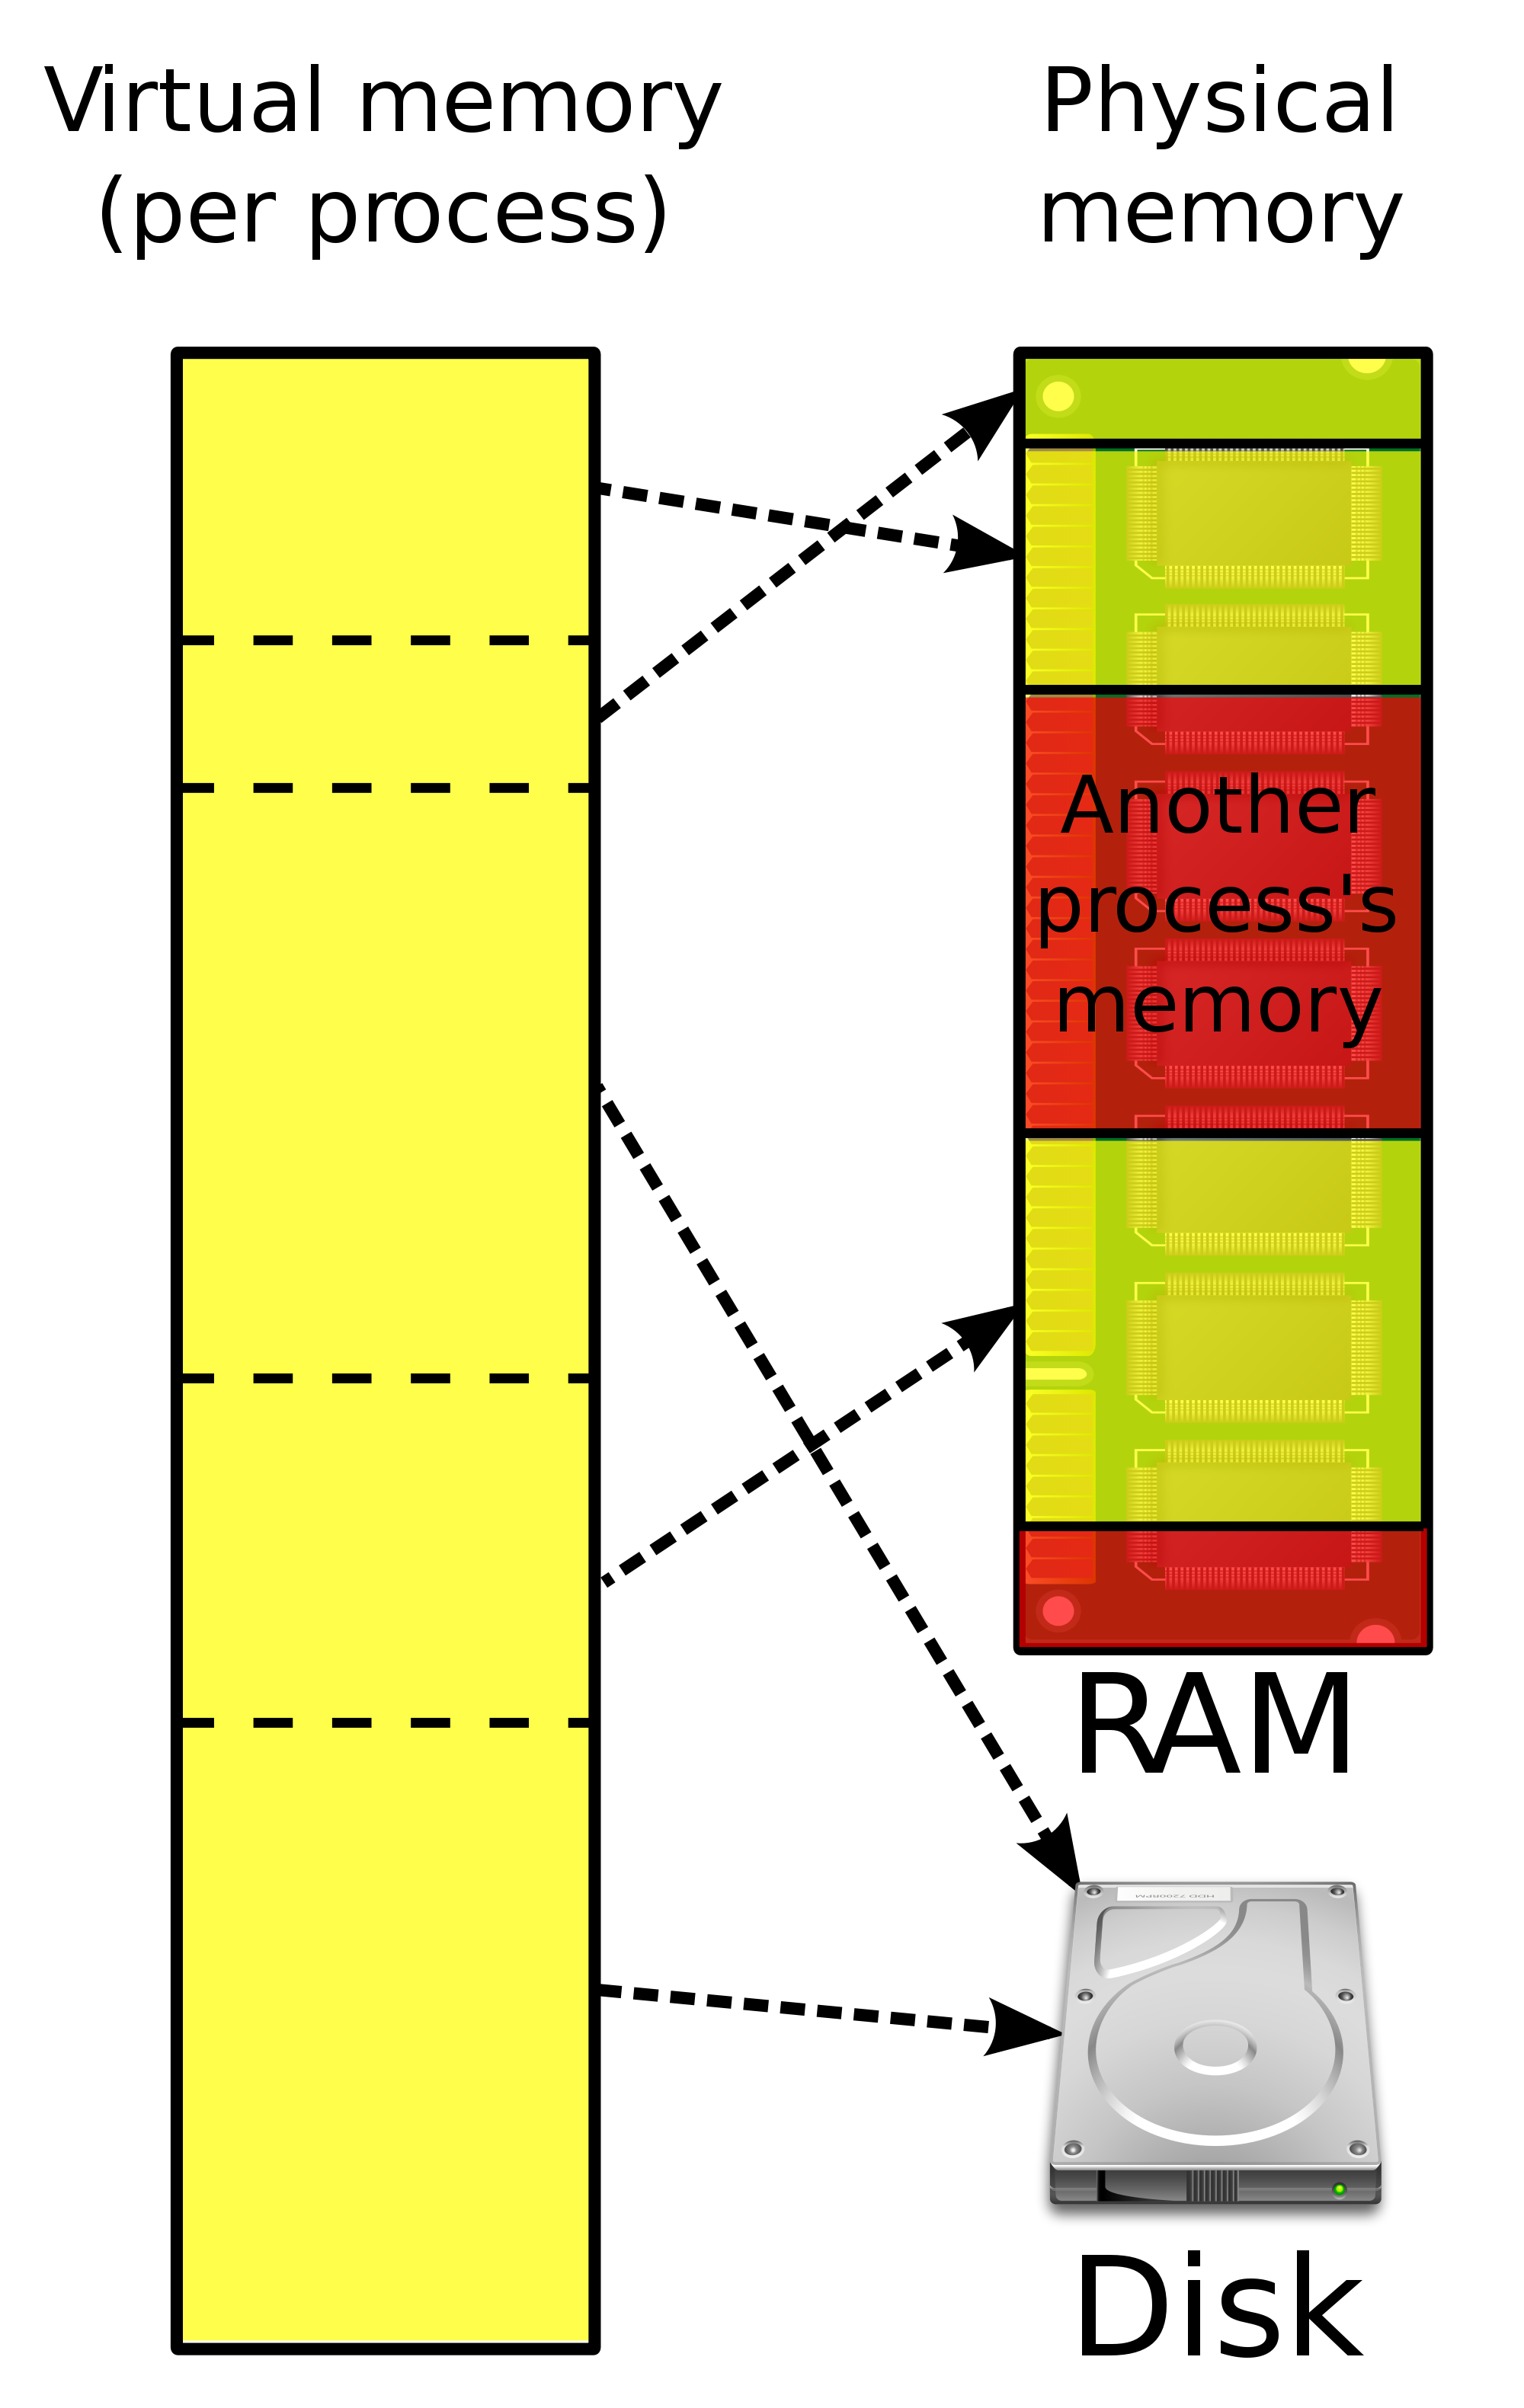
\includegraphics[width=1\textwidth, keepaspectratio=true]{images/vm.png}
      \end{figure}
    \end{column}

    \hfill
    \begin{column}{.8\textwidth}
      \begin{block}{}
        Page-based address translation hardware was originally designed to
        allow applications to use more memory than was physically present in
        the machine via demand paging.
      \end{block}\pause

      \begin{block}{}
        Paging almost never happens today, and large machines in the future
        are likely to have much more memory than can be represented in the
        virtual address space.
      \end{block}
    \end{column}
  \end{columns}
\end{frame}

%-------------------------------------------------------
\subsection{Network Stack}
%-------------------------------------------------------
\begin{frame}{Network Stack}{What's broken?}
%-------------------------------------------------------
  \begin{block}{}
    Network bandwidth to an adaptor is still increasing, but the speed of
    individual processing core is decreasing. \pause
  \end{block}

  \begin{block}{}
    De-multiplex network flows between end-system cores in the network
    interface controller hardware, using direct memory access (DMA) to write
    into a large number of different ring buffers.
  \end{block}

\end{frame}

\begin{frame}{Network Stack}{What's broken?}
  \begin{itemize}
    \item Slower cores relative to the network mean that every CPU cycle on the
          data path counts. This happened first in virtual machine monitors and
          spurred the adoption of technologies such as Single Root I/O
          virtualization. \pause
    \item NIC is no longer an interface. That makes forwarding decision at all
          layer of the traditional protocol stack. The role of the future OS is
          to implement the control plane for this switch.
  \end{itemize}
\end{frame}
%=======================================================
\section{Outlook}
%-------------------------------------------------------
\begin{frame}{Architecture}{Outlook}
  \begin{figure}[ht]
    \centering
    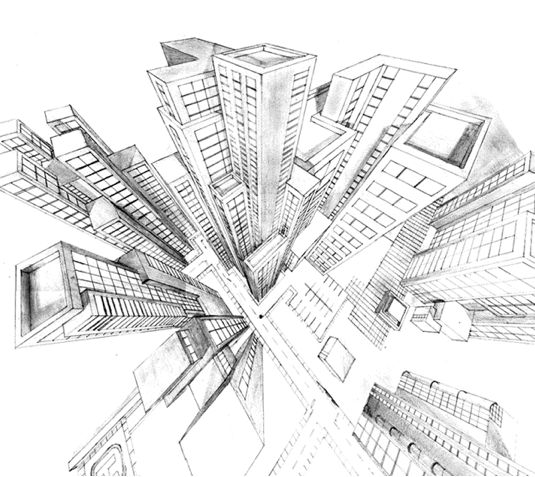
\includegraphics[width=0.7\textwidth, keepaspectratio=true]{images/outlook.jpg}
  \end{figure}
\end{frame}

\begin{frame}{Architecture}{Outlook}
%-------------------------------------------------------
  \begin{itemize}
    \item The future OS will be distributed in architecture. A single kernel
          isn't going to work with heterogeneous processors, memory that isn't
          accessible from all cores, or partial cache coherence. \pause
    \item There will be multiple kernels in a single machine, and some kind of
          message passing is inevitable. The result will be something between a
          single machine and traditional cluster. \pause
    \item The virtual machines or containers still need a hypervisor
          underneath, which is an OS\@. Moreover, we have already observed that
          application are increasingly parallel and distributed. \pause
    \item Containers are important: They make it easy to deploy traditional
          applications in virtualized traditional OS environment. Their low
          overhead allows applications to be restructured into much more
          scalable microservices, and enables a model of continuous
          re-engineering, refactoring, and redeployment. However, they don't
          yet adequately address the challenges of future hardware and scalable
          applications.
  \end{itemize}
\end{frame}

%-------------------------------------------------------
\subsection{Memory}
%-------------------------------------------------------
\begin{frame}{Memory}{Outlook}
%-------------------------------------------------------
  \begin{itemize}
    \item In most application scenarios, main memories will be very large and
          mostly persistent, and only cold date will be kept on disk. \pause
    \item Memory contents will persist across reboots, and files will be
          partially replaced with persistent in-memory data structure. \pause
    \item A future OS is going to have to provide something like sophisticated
          transactional facility to make persistent main memory usable.
          Sometimes remembering all the data is not desirable across reboot. \pause
    \item Instead of a virtual address space, applications will be given a much
          more explicit handle on the region of physical memory allocated to
          them, and more freedom in safely programming the MMU to exploit
          hardware translation feature from application runtime
  \end{itemize}
\end{frame}

%-------------------------------------------------------
\subsection{Network}
%-------------------------------------------------------
\begin{frame}{Network}{Outlook}
%-------------------------------------------------------
  \begin{block}{}
    OS software will increasingly get off the critical data path between
    application threads, replaced by sophisticated user-safe hardware
    multiplexing/de-multiplexing and filtering functionality, and library
    code to interface.
  \end{block}

  \begin{block}
    OS abstraction for this will resemble a more advanced form of those being
    formulated for SDN.
  \end{block}

\end{frame}

%-------------------------------------------------------
\subsection{Security}
%-------------------------------------------------------
\begin{frame}{Security}{Outlook}
%-------------------------------------------------------
  \begin{block}{}
    Low-level primitives that will scale up to very large numbers of principals
    seem like a good place to start;
  \end{block}
\end{frame}

%-------------------------------------------------------
\subsection{Applications}
%-------------------------------------------------------
\begin{frame}{Applications}{Outlook}
%-------------------------------------------------------
  \begin{block}{}
    The OS interface will have to change, but it is unreasonable to expect
    application developers to start afresh.
  \end{block}
\end{frame}

%-------------------------------------------------------
\section{Conclusion}
%-------------------------------------------------------
\begin{frame}{Conclusion}{}
%-------------------------------------------------------
\end{frame}

{\1
\begin{frame}[plain,noframenumbering]
  \finalpage{Thank you!}
\end{frame}}

\end{document}
